\onecolumn
\chapter{Auswertung}
% Liste der genutzer Formeln für die Fehlerrechnung
\section*{Fehlerrechnung}
Für die statistische Auswertung von $n$ Messwerten $x_i$ werden folgende Größen definiert \cite{errorSkript25}:
\begin{align}
    \bar{x} &= \frac{1}{n} \sum_{i=1}^{n} x_i \vphantom{\sqrt{\sum_i^n}^2} && \text{\textcolor{gray}{Arithmetisches Mittel}} \label{eq:arithmetisches_mittel} \\
    \sigma^2 &= \frac{1}{n-1} \sum_{i=1}^{n} (x_i - \bar{x})^2 \vphantom{\sqrt{\sum_i^n}^2} && \text{\textcolor{gray}{Variation}} \label{eq:variation} \\
    \sigma &= \sqrt{\frac{1}{n-1} \sum_{i=1}^{n} (x_i - \bar{x})^2} \vphantom{\sqrt{\sum_i^n}^2} && \text{\textcolor{gray}{Standardabweichung}} \label{eq:standardabweichung} \\
    \Delta \bar{x} &= \frac{\sigma}{\sqrt{n}} = \sqrt{\frac{1}{n(n-1)} \sum_{i=1}^n(\bar x - x_i)^2} \vphantom{\sqrt{\sum_i^n}^2} && \text{\textcolor{gray}{Fehler des Mittelwerts}} \label{eq:fehler_mittelwert} \\
    \Delta f &= \sqrt{\left(\frac{\partial f}{\partial x} \Delta x\right)^2 + \left(\frac{\partial f}{\partial y} \Delta y\right)^2} \vphantom{\sqrt{\sum_i^n}^2} && \text{\textcolor{gray}{Gauß’sches Fehlerfortpflanzungsgesetz für $f(x,y)$}} \label{eq:gauss_fehlfortpflanzung} \\
    \Delta f &= \sqrt{(\Delta x)^2 + (\Delta y)^2} \vphantom{\sqrt{\sum_i^n}^2} && \text{\textcolor{gray}{Fehler für $f = x + y$}} \label{eq:fehler_summe} \\
    \Delta f &= |a| \Delta x \vphantom{\sqrt{\sum_i^n}^2} && \text{\textcolor{gray}{Fehler für $f = ax$}} \label{eq:fehler_proportional} \\
    \frac{\Delta f}{|f|} &= \sqrt{\left(\frac{\Delta x}{x}\right)^2 + \left(\frac{\Delta y}{y}\right)^2} \vphantom{\sqrt{\sum_i^n}^2} && \text{\textcolor{gray}{relativer Fehler für $f = xy$ oder $f = x/y$}} \label{eq:relativer_fehler} \\
    \sigma &= \frac{|a_{lit} - a_{gem}|}{\sqrt{\Delta a_{lit}^2 + \Delta a_{gem}^2}} \vphantom{\sqrt{\sum_i^n}^2} && \text{\textcolor{gray}{Berechnung der signifikanten Abweichung}} \label{eq:signifikante_abweichung}
\end{align}

\twocolumn

\section{Berechnung des Wasserwertes}
Wir beginnen mit der \hyperref[eq:wasserwert]{Berechnung des Wasserwertes}. 
Hierfür benötigen wir zwei Referenztemperaturen. Wir nutzen einmal die Zimmertemperatur $T_2 = 25,1 ^\circ C$. Dabei gehen wir von einer Ungenauigkeit des Thermometers von $1^\circ C$ aus.
Wichtig für die Rechnung sind die Werte aus \hyperref[Prtokoll]{Tabelle 2 des Protokolls}. Dort sind zwei Messreihen aufgeführt.
Die zweite Messreihe wurde durchgeführt, da wir bei der ersten Messreihe die Durchführung nicht genau genug beachtet hatten. Die grauen Werte entsprechen dabei immer der ersten Messreihe.
In der Gleichung des Wasserwertes kommt die spezifische Wärmekapazität des Wassers vor. Dafür nutzen wir den Literaturwert
$c_w = (4,186 \pm 0,004) \frac{J}{g \cdot K}$. Zur Bestimmung der Masse des Wassers $m_w$ wurde das Kalorimeter einmal leer $m_l$ und einmal mit Wasser gefüllt $m_v$ gewogen.
Zieht man die Differenz beider, so erhält man eine Masse von:
\begin{equation}
    m_w = 354,2 \, \mathrm{g}.
\end{equation}

Diesen Wert können wir jedoch nicht einfach so übernehmen; wir müssen noch seine Ungenauigkeit bestimmen. Die Messunsicherheit der Waage liegt bei $\Delta m = 0,1 \, \mathrm{g}$. Dieser Fehler gilt für beide Massen.
Über die \hyperref[eq:gauss_fehlfortpflanzung]{Gauß'sche Fehlerfortpflanzung} ergibt sich somit eine Ungenauigkeit von
\begin{equation}
    \Delta m_w = \sqrt{\Delta m_l^2 + \Delta m_v^2} = 0,141 \, \mathrm{g}.
\end{equation}

Fügen wir dies zusammen, ergibt sich eine Wassermasse von
\begin{equation}
    m_w = (354,2 \pm 0,14) \, \mathrm{g}.
\end{equation}

Bei der zweiten Messreihe haben wir extra darauf geachtet, möglichst exakt die gleiche Masse zu erreichen. 
Für den Wasserwert benötigen wir jedoch noch einen zweiten Referenzwert, $T_1$.
Das Thermometer weist einen Fehler von \(\pm(0{,}3\,\% + 1\,\mathrm{^\circ C})\) auf. Systematische Fehler, die absolute Temperaturmessungen verzerren, sind darin vermutlich bereits berücksichtigt. Da in diesem Versuch nur Temperaturdifferenzen relevant sind, auf die systematische Abweichungen kaum Einfluss haben, kann man hier ausschließlich den relativen Fehler von $0{,}3\,\%$ des Messwertes ansetzen.
Dies kann jedoch nicht mit absoluter Sicherheit gesagt werden. Trotzdem wurde dies so gemacht, da sonst die \hyperref[fig:temp_against_time]{Abbildung [\ref*{fig:temp_against_time}]} keinen Sinn für die graphische Bestimmung ergeben würde.
Der Wert $T_1$ ist dem \hyperref[Prtokoll]{Protokoll, Tabelle 2} zu entnehmen:
\begin{align}
    T_1 = (50,0 \pm 0,15)^\circ C \\ 
    \notag \textcolor{gray}{T_1 = (50,5 \pm 0,15)^\circ C}.
\end{align}

Der \hyperref[fig:temp_against_time]{Abbildung \ref*{fig:temp_against_time}} sind die Werte
\begin{align}
    \overline{T_A} = 49,09^\circ C  \text{ und}\\
    \overline{T_F} = 49,18^\circ C
\end{align}
zu entnehmen. Die Ungenauigkeit berechnet sich zu
\begin{equation}
    \Delta \bar{T} = \left| \overline{T_A} - \overline{T_F} \right| = 0,09 \, \mathrm{^\circ C}.
\end{equation}

Zusammengefasst ergibt sich:
\begin{equation}
    \bar{T} = (49,09 \pm 0,09) ^\circ C.
\end{equation}

Mit diesen Werten können wir nun den Wasserwert berechnen:
\begin{equation}
    W = 354,2 \cdot 4,186 \frac{0,91}{23,99} = 56,24176 \frac{J}{K}.
\end{equation}

Nun muss noch die Ungenauigkeit bestimmt werden. Wir nutzen erneut die \hyperref[eq:gauss_fehlfortpflanzung]{Gauß'sche Fehlerfortpflanzung}:
\begin{equation}
    \Delta W = 
    \sqrt{
    \begin{aligned}
    &\left( c_W \frac{T_1 - \overline{T}}{\overline{T} - T_2} \Delta m_W \right)^2 \\
    &+ \left( m_W \frac{T_1 - \overline{T}}{\overline{T} - T_2} \Delta c_W \right)^2 \\
    &+ \left( m_W c_W \frac{1}{\overline{T} - T_2} \Delta T_1 \right)^2 \\
    &+ \left( - m_W c_W \frac{T_1 - \overline{T}}{(\overline{T} - T_2)^2} \Delta T_2 \right)^2 \\
    &+ \left( m_W c_W \frac{T_2 - T_1}{(\overline{T} - T_2)^2} \overline{\delta t} \right)^2
    \end{aligned}
    }
    \label{eq:deltaW}
\end{equation}

Setzt man alle Werte ein, ergibt sich
\begin{equation}
    \Delta W = 11,1714 \frac{J}{K}.
\end{equation}

Zusammengefasst ergibt sich das Ergebnis:
\begin{equation}
    \boxed{W = (56,24 \pm 11,17) \frac{J}{K}}
\end{equation}
\begin{equation*}
    \textcolor{gray}{
        \boxed{W = (9 \pm 54) \frac{J}{K}}
    }
\end{equation*}
Es ist sehr eindeutig, dass die erste Messreihe misslungen ist und keinen Sinn ergibt.

\onecolumn
\begin{figure}
    \centering
    \includegraphics[width=\textwidth, page=4]{Protokolle/\versuchsnummer/Chapter/Messprotokoll.pdf}
    \caption{Graphischebestimmung des Wasserwertes. Dabei sind zwei Messreihen vermerkt, die Rote (unten) ist die korrigierte, und desswen Wasserwert im folgenden verwendet wird. Die blaue Messreihe dient nur als Vergleich und soll zeigen, dass die Verbesserte Messreihe, tatsächlich besser war.}
    \label{fig:temp_against_time}
\end{figure}
\twocolumn



\section{Berechnung der spezifischen Wärmekapazität im Kalorimeter}
Wir bestimmen nun die spezifische Wärme der drei Probematerialien (Aluminium (Al), Blei (Pb) und Graphit (C-Verbindung)). 
Zunächst müssen wir jedoch die tatsächliche Temperatur des kochenden Wassers bestimmen, da die $100^\circ C$ nur bei Normaldruck $p_0 = 1013 \, \mathrm{hPa}$ gelten.
Daher berechnen wir unsere tatsächliche Temperatur:
\begin{equation}
    T_1(p) = 100^\circ C + 0,0276 \frac{^\circ C}{\mathrm{hPa}} \cdot (p-p_0).
    \label{eq:temp_corecctur}
\end{equation}

Wir haben einen Luftdruck von $P = 1001,2 \, \mathrm{hPa}$ abgelesen und gehen von einer Ungenauigkeit von $\Delta p = 0,5 \, \mathrm{hPa}$ aus.
Setzt man diese Werte in die \hyperref[eq:temp_corecctur]{Gleichung} ein, ergibt sich:
\begin{equation}    
    T_1 = 99,674 ^\circ C.
\end{equation}

Die Ungenauigkeit berechnet sich über:
\begin{equation}
    \Delta T_1 = 0,0276 \frac{^\circ C}{\mathrm{hPa}} \cdot \Delta p = 0,0138,
\end{equation}

somit ergibt sich ein Ergebnis von
\begin{equation}
    \underline{T_1 = (99,674 \pm 0,014)^\circ C}.
\end{equation}

Wir berechnen nun die \hyperref[eq:spezifische_waermekapazitaet]{spezifische Wärme}. Dabei muss auch die Ungenauigkeit über die \hyperref[eq:gauss_fehlfortpflanzung]{Gauß'sche Fehlerfortpflanzung} bestimmt werden:

\begin{equation}
    \Delta c_x = 
    \sqrt{ 
    \begin{aligned}
    &   \left( \frac{c_W ( \overline{T} - T_2)}{T_1 - \overline{T}} \frac{1}{m_x} \Delta m_W \right)^2 \\
    & + \left( \frac{m_W (\overline{T} - T_2)}{T_1 - \overline{T}} \frac{1}{m_x} \Delta c_W \right)^2 \\
    & + \left( \frac{\overline{T} - T_2}{(T_1 - \overline{T}) m_x} \Delta W \right)^2 \\
    & + \left( \frac{c_x \Delta m_x}{m_x} \right)^2 \\
    & + \left( - \frac{(T_1 - T_2)(c_W m_W + W)}{m_x (T_1 - \overline{T})^2} \overline{\delta t} \right)^2 \\
    & + \left( \frac{(c_W m_W + W)}{m_x (\overline{T} - T_2)} \Delta T_1 \right)^2 \\
    & + \left( \frac{c_x \Delta T_2}{\overline{T} - T_2} \right)^2
    \end{aligned}
    }
    \label{eq:deltacx}
\end{equation}

Für $\Delta T_1$ nutzen wir die Angaben des Thermometerherstellers: $\Delta T_1 = \pm(0,3\% + 1^\circ C)$.
Die Ergebnisse stellen wir \hyperref[tab:waermekapazitaeten]{tabellarisch (\ref*{tab:waermekapazitaeten})} dar.

\subsection*{Vergleich: Messwert, Literaturwert und Dulong-Petit}
In diesem Abschnitt wollen wir untersuchen, wie stark unsere Messwerte von den Literaturwerten abweichen und wie zuverlässig das Gesetz von Dulong-Petit angewendet werden kann.
Das Gesetz besagt, dass jeder Körper über
\begin{equation}
    c_\mathrm{mol} = 3 \cdot R \approx 24,94 \frac{\mathrm{J}}{\mathrm{mol \cdot K}}
\end{equation}
beschrieben werden kann, wobei $R$ die universelle Gaskonstante ist. Die Ergebnisse halten wir wieder \hyperref[tab:e_tab_abw]{tabellarisch (\ref*{tab:e_tab_abw})} fest.

\onecolumn
\begin{table}[h!]
    \centering
    \begin{tabular}{l | l | l | l}
        \toprule
        Größe & Graphit & Blei & Aluminium \\
        \hline
        $T_2 [^\circ C]$ & $33,5 \pm 1,1$ & $30,8 \pm 1,1$ & $25,5 \pm 1,1$ \\
        $\overline{T} [^\circ C]$ & $36,6 \pm 0,09$ & $33,3 \pm 0,09$ & $30,5 \pm 0,1$ \\
        $m_w [g]$ & $372,2 \pm 1$ & $373 \pm 1$ & $373,2 \pm 1$ \\
        $m_x [g]$ & $122,2 \pm 1$ & $618,3 \pm 1$ & $148,9 \pm 1$ \\
        $M [\mathrm{g/mol}]$ & $12,01$ & $207,2$ & $26,98$ \\
        \midrule
        $c_x [\mathrm{J/g \cdot K}]$ & $0,649 \pm 0,219$ & $0,10 \pm 0,04$ & $0,65 \pm 0,16$ \\
        $c_\mathrm{mol} [\mathrm{J/mol \cdot K}]$ & $8 \pm 3$ & $20 \pm 9$ & $19 \pm 4$ \\
        \bottomrule
    \end{tabular}
    \caption{Messwerte und Unsicherheiten für Graphit, Blei und Aluminium. Dabei gilt $c_{\mathrm{mol},x} = M \cdot c_x$, $\Delta c_{\mathrm{mol},x} = M \cdot \Delta c_x$}
    \label{tab:waermekapazitaeten}
\end{table}

\begin{table}[h!]
    \centering
    \begin{tabular}{l | l | c | c c}
        \toprule
        Material & $c_{x,\mathrm{gem}} [\mathrm{J/g \cdot K}]$ & $c_{x,\mathrm{lit}} [\mathrm{J/g \cdot K}]$ & Abweichung \\
        \hline
        Graphit & $0,649 \pm 0,219$ & 0,709 & $0,27\sigma$ & $72,1\%$\\
        Blei & $0,10 \pm 0,04$ & 0,129 & $0,72\sigma$ & $10,9\%$\\
        Aluminium & $0,65 \pm 0,16$ & 0,90 & $1,19\sigma$ & $78,6\%$\\
        \midrule
        \midrule
        Material & $c_{x,\mathrm{mol,gem}} [\mathrm{J/mol \cdot K}]$ & $c_{x,\mathrm{lit}} [\mathrm{J/mol \cdot K}]$ & Abweichung \\
        \hline
        Graphit & $8 \pm 3$ & 24,94 & $6,52\sigma$ & $31,3\%$\\
        Blei & $20 \pm 9$ & 24,94 & $0,52\sigma$ & $81,9\%$\\
        Aluminium & $19 \pm 4$ & 24,94 & $1,34\sigma$ & $76,5\%$\\
        \bottomrule
    \end{tabular}
    \caption{Vergleich der gemessenen Werte mit Literaturwerten und Dulong-Petit.}     
    \label{tab:e_tab_abw}
\end{table}
\twocolumn






\section{Berechnung der spezifischen Wärme im Flüssigstickstoff}
Wir wollen erneut die spezifische Wärmekapazität der drei Proben bestimmen, jedoch dieses Mal über (kalten) Flüssigstickstoff.
Dafür greifen wir auf \hyperref[eq:stickstoff_cx]{Gleichung (\ref*{eq:stickstoff_cx})} zurück. 
Die Verdampfungswärme des flüssigen Stickstoffs ist mit $Q_V = 199 \frac{J}{g}$ und seine Temperatur mit $T_2 = -195,8^\circ C$ gegeben.
Zu diesem Zeitpunkt lag die Raumtemperatur bei $T_1 = (26,1 \pm 1)^\circ C$. 
Die Differenz der beiden Temperaturen ergibt $\overline{T} = T_1 - T_2 = (221,9 \pm 1,0)^\circ C$.
Die Ungenauigkeit von $c_x$ ergibt sich über die \hyperref[eq:gauss_fehlfortpflanzung]{Gauß'sche Fehlerfortpflanzung} zu:
\begin{equation}
    \frac{\Delta c_x}{c_x} =
    \sqrt{
    \left( \frac{\Delta m_s}{m_s} \right)^2
    + \left( \frac{\Delta m_x}{m_x} \right)^2
    + \left( \frac{\Delta T_1}{\overline{T}} \right)^2
    }
    \label{eq:d_c-x_s}
\end{equation}

Der Fehler für die $c_{x,\mathrm{mol}}$-Werte wird analog berechnet.
Die Ergebnisse sind in \hyperref[tab:e_st]{Tabelle (\ref*{tab:e_st})} dargestellt.
Es wurden zwei Messreihen durchgeführt, einmal mit den leichten und einmal mit den schweren Probekörpern. 

\begin{table}[h!]
    \onecolumn
    \centering
    \begin{tabular}{l | l | l | c | c}
        \toprule
        Material & $m_x [g]$ & $m_V [g]$ & $c_x [\frac{J}{g K}]$ & $c_{x,\mathrm{mol}} [\frac{J}{g K}]$ \\
        \hline
        Graphit & $44,7 \pm 1$ & $20,3 \pm 0,14$ & $(0,407 \pm 0,010)$ & $(4,891 \pm 0,117)$ \\
        Blei & $138,3 \pm 1$ & $19 \pm 0,14$ & $(0,1232 \pm 0,0014)$ & $(25,53 \pm 0,29)$ \\
        Aluminium & $34,9 \pm 1$ & $28,9 \pm 0,14$ & $(0,7426 \pm 0,0218)$ &$(20,0 \pm 0,6)$ \\
        \midrule
        Graphit & $122,2 \pm 1$ & $63,2 \pm 0,14$ & $(0,464 \pm 0,004)$ & $(5,57 \pm 0,05)$ \\
        Blei & $618,3 \pm 1$ & $90,3 \pm 0,14$ & $(0,1310 \pm 0,0007)$ & $(27,14 \pm 0,14)$ \\
        Aluminium & $148,9 \pm 1$ & $112 \pm 0,14$ & $(0,675 \pm 0,006)$ & $(18,20 \pm 0,15)$\\
        \bottomrule
    \end{tabular}
    \caption{Messwerte und berechnete Werte: verdampfte Stickstoffmasse, spezifische Wärmekapazität $c_x$ und molare Wärmekapazität $c_{x,\mathrm{mol}}$.}     
    \label{tab:e_st}
    \twocolumn
\end{table}

\onecolumn
\twocolumn
\newpage
\section{Spezifische Molwärmen und Debye-Temperatur}
Wir wollen nun die spezifischen Molwärmen $c_{x,\mathrm{mol}}$ untereinander vergleichen. Dafür definieren wir das Verhältnis als Quotienten:
\begin{equation}
    q := \frac{c_{x,\mathrm{mol},N_2}}{c_{x,\mathrm{mol},H_2O}}.
\end{equation}

Die Ungenauigkeit berechnet sich über die \hyperref[eq:gauss_fehlfortpflanzung]{Gauß'sche Fehlerfortpflanzung} zu 
\begin{equation}
    \Delta q = \sqrt{\left(\frac{\Delta c_{x,\mathrm{mol},N_2}}{c_{x,\mathrm{mol},N_2}}\right)^2 + \left(\frac{\Delta c_{x,\mathrm{mol},H_2O}}{c_{x,\mathrm{mol},H_2O}}\right)^2} \cdot q.
\end{equation}

Für die schweren Proben im Stickstoff ergeben sich:
\begin{align}
    &q_{Graphit,s} = 0,7 \pm 0,4 \\
    &q_{Blei,s} = 1,4 \pm 0,5 \\
    &q_{Aluminium,s} = 0,9579 \pm 0,2107
\end{align}

Für die leichten Proben:
\begin{align}
    &\boxed{q_{Graphit,l} = 0,6 \pm 0,4} \\
    &\boxed{q_{Blei,l} = 1,3 \pm 0,5} \\
    &\boxed{q_{Aluminium,l} = 1,0526 \pm 0,2127}.
\end{align}

Mit diesen Größen können nun graphisch über die bereitgestellte Debye-Tabelle die Werte bestimmt werden.
Dies wurde für die schweren und die leichten Proben durchgeführt. Die graphische Auswertung für die leichten Proben ist in \hyperref[img:graphisch_leicht]{Abbildung (\ref*{img:graphisch_leicht})} zu sehen, für die schweren Proben in \hyperref[img:graphisch_schwer]{Abbildung (\ref*{img:graphisch_schwer})}.

Die Ergebnisse sind in \hyperref[tab:e_finn_will_nicht_mehr]{Tabelle (\ref*{tab:e_finn_will_nicht_mehr})} dargestellt. Die abgelesenen Debye-Temperaturen sind mit $T_D$ bezeichnet.
Die leichten Werte (l) stehen in der oberen Spalte, die schweren Werte (s) darunter.

Bei Blei konnte der >>tatsächliche<< Wert leider nicht eingezeichnet werden, nur der Maximalwert war auf der Skala auffindbar.
Daher wurde vereinfacht angenommen, dass der Absolute Nullpunkt (0 K) die untere Grenze und der Maximalwert die obere Grenze darstellt; das Mittel dieser beiden Werte wurde als >>eigentlicher<< Wert genommen. Dies ist selbstverständlich eine starke Vereinfachung.
Außerdem wurde die \hyperref[eq:signifikante_abweichung]{signifikante Abweichung (\ref*{eq:signifikante_abweichung})} bestimmt.


\begin{table}[h!]
    \centering
    \begin{tabular}{l | l | l | c }
        \toprule
        Material (l) & $T_D [K]$ & $T_{D,\mathrm{lit}} [K]$ & Abweichung \\
        \hline
        Aluminium & $100 \pm 50$ & 430 & $6,6\sigma$ \\
        Blei (max) & $200 \pm 200$ & 95 & $0,525\sigma$ \\
        Graphit & $750 \pm 80$ & 2230 & $18,5\sigma$ \\
        \midrule
        Material (s) & $T_D [K]$ & $T_{D,\mathrm{lit}} [K]$ & Abweichung \\
        \hline
        Aluminium & $250 \pm 35$ & 430 & $5,14\sigma$ \\
        Blei (max) & $125 \pm 125$ & 95 & $0,24\sigma$ \\
        Graphit & $275 \pm 75$ & 2230 & $26,1\sigma$ \\
        \bottomrule
    \end{tabular}
    \caption{Auflistung der gemessenen Debye-Temperaturen $T_D$ für leichte (l) und schwere (s) Proben sowie Vergleich mit Literaturwerten.}     
    \label{tab:e_finn_will_nicht_mehr}
\end{table}

\onecolumn
\begin{figure}[t!]
    \raggedright
    \hspace*{-2.2cm}
    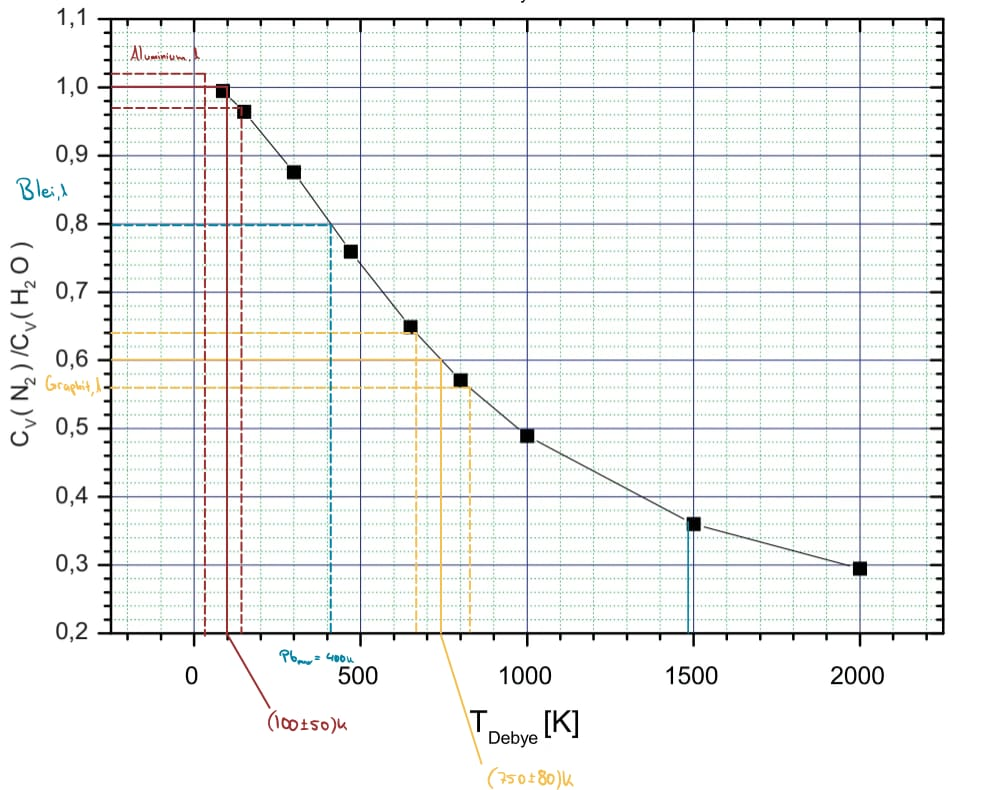
\includegraphics[width=1.3\textwidth]{img/\versuchsnummer/leicht.jpg}
    \caption{Debye-Tabelle mit den eingezeichneten Werten für die leichten Proben}
    \label{img:graphisch_leicht}
\end{figure}

\begin{figure}[b!]
    \raggedright
    \hspace*{-2.2cm} 
    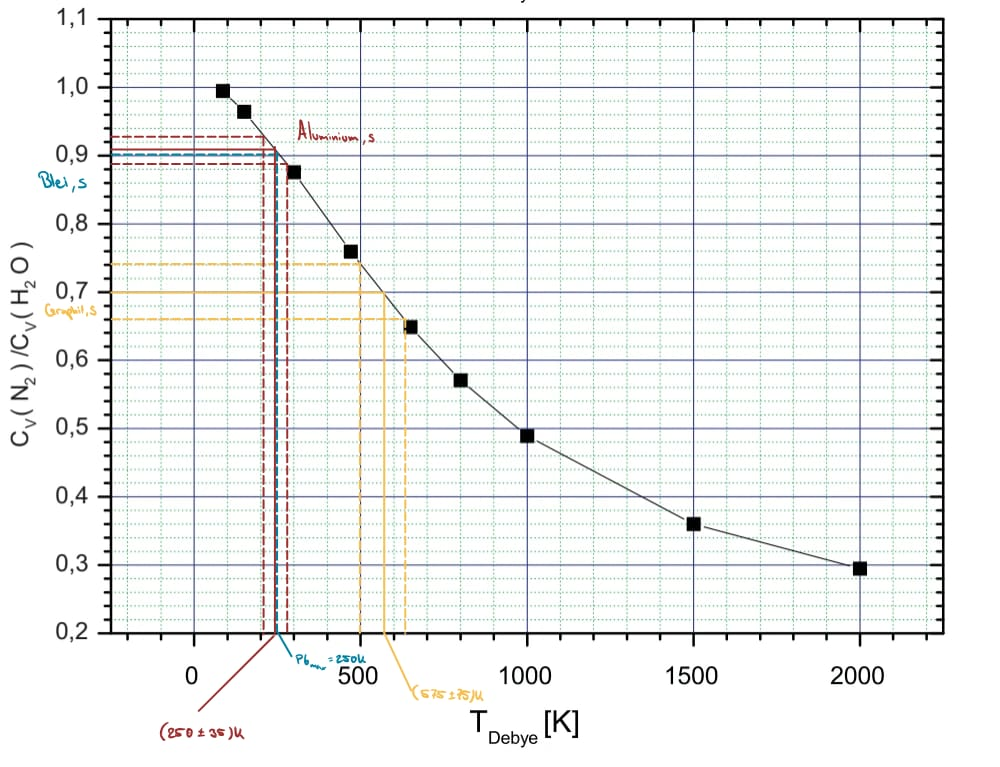
\includegraphics[width=1.3\textwidth]{img/\versuchsnummer/schwer.jpg}
    \caption{Debye-Tabelle mit den eingezeichneten Werten für die schweren Proben}
    \label{img:graphisch_schwer}
\end{figure}
\twocolumn
